\chapter{Design der Bibliothek}
\label{cha:design_der_bibliothek}

Diese Kapitel beschäftigt sich mit dem Design der Bibliothek, welche im Zuge dieser Arbeit erstellt wurde. Zuerst werden die Abhängigkeiten zu anderen Bibliotheken  \linebreak beschrieben und für diese argumentiert. Danach wird auf die Architektur der Bibliothek eingegangen. Die Sammlung und Berechnung von Metriken wird beschrieben. Zuletzt wird noch das Design der Diagramm-Komponenten erläutert.


\section{Abhängigkeiten auf andere Bibliotheken}
\label{sec:base_library}

% Gewählte Technologien zur Umsetzung
%   - maptlot
%   - numpy
Scikit-charts wird basierend auf Matplot, Numpy, Pandas und Scikit-learn entwickelt. Dabei wird bei den Versionsnummern grundsätzlich von der neuesten Version ausgegangen. Als Alternative zu Matplot wurde kurzzeitig Seaborn in Erwägung gezogen. Die zusätzliche Unterstützung für angehängte Diagramme an den Achsen würde die Implementierung des Schnittdiagramms vereinfachen. Das alleine rechtfertigt jedoch nicht die Abhängigkeit zur Bibliothek.\\\\
\noindent Numpy \footnote{https://numpy.org/} wird in der Bibliothek zur optimierten Berechnung der Metriken benötigt. Es handelt sich dabei um den De-facto-Standard zum effizienten Rechnen von N-dimensionalen Arrays in Python. Numpy-Arrays bieten außerdem weiter Funktionen um die Verwendung von Arrays zu vereinfachen. Grundlegende Arithmetische Funktionen können\linebreak direkt auf Numpy-Arrays angewandt werden. Zusätzlich werden verschiedene statistische Funktionen zur Auswertung angeboten.\\\\
\noindent Die Pandas-Bibliothek bietet eine Datenstruktur sowie Funktionen zur Verwaltung von tabellarischen Daten. Diese wird zentral bei der Berechnung und Verwaltung der\linebreak Metriken verwendet.\\\\
\noindent Scikit-learn wird in der Bibliothek nur zur Berechnung der \emph{partial dependence}\footnote{https://scikit-learn.org/stable/modules/partial\_dependence.html\#partial-dependence-plots} (Abschnitt \ref{fig:partial_dependence}) aus einem Modell benötigt. Dadurch ist das Schnittdiagramm als einziges auf Scikit-learn Modelle beschränkt. Sonstige Diagramme sind von Scikit-learn unabhängig. In diesen wird nur ausgegangen, dass die verwendeten Objekten der formellen Definition laut Dokumentation entspricht. Durch diesen Ansatz kann die Bibliothek auch mit anderen Implementierungen von Regressionsmodellen verwendet werden.\\\\
\noindent Zuletzt wird noch eine Abhängigkeit Pytest\footnote{https://docs.pytest.org/en/7.4.x/} benötigt. Diese Bibliothek wird für die Entwicklung von Tests in der Bibliothek verwendet.

\section{Sammeln von Metriken aus Modellen}
\label{sec:design_sammeln_metriken}

Das Sammeln der Metriken aus einem Modell soll mithilfe eines einzelnen Funktionsaufrufs möglich sein. Für die Berechnung werden zwei Werte benötigt. Zum Einen eine Referenz auf die \emph{predict}-Funktion eines \emph{predictors} (Abschnitt \ref{sec:scikit-learn}). Zum Anderen der originale Datensatz, aus welchem das Modell erstellt wurde.  Wie in Scikit-learn wird dieser als X- und Y-Arrays übergeben. Das Ergebnis wird als ein Pandas-Dataframe\linebreak zurückgegeben. Dieser enthält alle Metriken, welche zur finalen Visualisierung notwendig sind.

\begin{PythonCode}
PredictFunction: TypeAlias = Callable[[Tuple[float]], float]

def create_metrics(
        x: Union[np.ndarray[float], list[list[float]]],
        y: Union[np.ndarray[float], list[float]],
        predict: PredictFunction
) -> DataFrame:
\end{PythonCode}

% Wie werden die gesammelten Daten verwaltet?
%   - Pandas-Dataframe verwenden und als Argument zurückgeben (Argumentieren warum)
% Warum?
%   - Direkter Zugriff auf gesammte Metrik / einzelne Werte
%   - Flexibel -> Hinzufügen / Entfernen von Metriken
%   - Einfache erstellung berechneter Spalten
%   - Existierende Funktionen zum Filtern + Sortieren der Werte
\noindent Ein DataFrame bietet einige Vorteile gegenüber einer eigens implementierten Datenstruktur. Sie unterstützt einen indizierten Zugriff. Damit können sowohl einzelne Einträge als auch alle Werte einer Metrik ausgewählt werden. Weiters ist die Datenstruktur flexibel. Sie kann noch nach der Erstellung um Spalten erweitert werden. Die Erstellung von berechneten Spalten aus anderen Metriken wird ebenfalls unterstützt. Außerdem existieren bereits Funktionen zum Filtern und Sortieren der Daten.\\\\

%   - Argumentation: Nutzung von Funktionsreferenz +  Beschreibung von X / Y
\noindent Wie bereits angemerkt wird durch die Übergabe einer einzelnen \emph{predict}-Funktion die Flexibilität der Berechnung erhöht. Typinformationen aus Scikit-learn werden nicht benötigt. Es werden außerdem beliebige Modelle anderer Bibliotheken unterstützt. Möglicherweise inkompatible Funktionen können dabei über eigene Lambda-Funktionen an das Interface angepasst werden. Durch dieses Design wird ebenfalls die Testbarkeit der Funktion erleichtert. Bei einer Abhängigkeit auf ein Scikit-learn Modell würde ein\linebreak eigenes Mocking-Framework benötigt werden.\\\\

% Metriken welche gesammelt werden?
%       - Metriken aus Kapitel über Heuristiclab
%       - Accuracy pro Wert ausrechnen für REC-Nachstellung
%           - https://scikit-learn.org/stable/modules/model_evaluation.html#roc-auc-binary
%       - Deviation für REC Kurve
\noindent Die zurückgegebenen Metriken im Dataframe entsprechen den Metriken im Abschnitt \ref{sec:design_sammeln_metriken}. Die Berechnung der einzelnen Metriken, sowie deren Namen für den Spaltenzugriff sind nachfolgend aufgelistet.

\pagebreak

% Wie werden die Metriken berechnet?
\begin{description}
\item[index] \emph{i}\hfill\newline
\emph{i} entspricht dem aktuellen Index einer Zeile im Datensatz.
\item[x0 ... xn] \emph{x[i][n]}\hfill\newline
\emph{x} entspricht den Werten der Einflussvariablen für die predict-Funktion.\newline \emph{n} entspricht dem Index einer Einflussvariable.
\item[target] \emph{y[i]}\hfill\newline
\emph{y} entspricht den Zielwerten aus dem Datensatz.
\item[prediction] \emph{predict(x[i])} \hfill\newline
\emph{prediction} entspricht Funktion eines Modells, welche für Werte der Einflussvariablen eine Vorhersage generiert.
\item[residual] \emph{target - prediction}\hfill
\item[relative\_error] \emph{residual / target}\hfill
\end{description}

\section{Aufbau der Diagramme}
\label{sec:design_aufbau_diagramme}
% Wie werden einzelne Diagramme umgesetzt aus Metriken (Allgemein)?

% Allgemeiner Aufbau + Features dieser Klassen / Funktionen 
%       - Basisklasse für Implementerierung + Funktion für erstellung aus Daten & Predict
%       - Zurückgeben von Plot-Objekt damit user anpassen kann (Labels, ...)
Jedes der Diagramme besitzt den selben Aufbau. Es existiert eine Klasse, welche die Funktionalitäten des Diagramm implementiert. Die Klasse dient dabei sowohl zur Strukturierung des Codes, als auch zum Halten aller benötigten Referenzen an einem Ort. Eine weitere Funktion mit dem Namen des Diagramms dient zur Instanziierung der Klasse. Die übergebenen Argumente werden darin für die Klasse vorbereitet und an den Konstruktor übergeben. Zurückgegeben wird am Ende nur das eigentliche Figure-Objekt. Die konkrete Implementierung der Diagramme bleibt dadurch für die Benutzer:innen der Bibliothek verborgen. Über das zurückgegebene Figure-Objekt kann das Diagramm angezeigt werden. Mithilfe von Matplot lassen sich außerdem weitere visuelle Anpassungen über das Figure-Objekt am Diagramm vornehmen.

\begin{figure}[H]
    \centering
    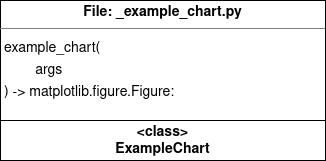
\includegraphics[width=0.4\textwidth]{images/uml_chart_design.png}
    \caption{Grundlegende Struktur einer Diagramm-Implementierung}
    \label{fig:uml_chart_design}
\end{figure}

%       - Compositions-Basiert (Allgemeine Fuhktionen wie Zoom select, etc) + Warum keine Vererbung?
\noindent Um gemeinsame Funktionalitäten zwischen den Diagrammen zu teilen wird mit Komposition gearbeitet. Funktionalitäten wie UI-Elemente werden dabei als eine unabhängige Komponente implementiert. In den Diagrammklassen selbst werden diese Komponenten dann angewandt. Vererbung wurde hierbei nicht gewählt, wegen den großen funktionalen Unterschieden zwischen den Diagrammen. Die Implementierung der Hilfsfunktionen und Klassen erfolgt dabei je nach Bedarf.